% interim.tex	K. J. Turner	10/09/13

% Interim Project Report Outline

\documentclass[a4paper,11pt]{report}

\usepackage{interim}
\usepackage{identfirst}
\usepackage{graphicx}
\usepackage{chngcntr}
\counterwithout{figure}{chapter}

\title{Smart contracts on Hyperledger}			% Insert your project title

\author{
{Yordan Gospodinov} \\
{\small{Supervised by Dr. Andrea Bracciali}}
}			% Insert your name

\renewcommand{\baselinestretch}{1.1}
\date{October 2018}			% Insert your submission date
\begin{document}

\maketitle				% Uncomment for final draft

\pagenumbering{arabic}

\tableofcontents
\thispagestyle{empty}
\clearpage

\setcounter{page}{1}
%%%%%%%%%%%%%%%%%%%%%%%%%%%%%%%%% Introduction %%%%%%%%%%%%%%%%%%%%%%%%%%%%%%%%%

\chapter{Introduction}

\label{introduction}

Recently a new technology emerged into the world that is called blockchain. The idea is that it is a distributed decentralized database of blocks of transactions. The reason why I find it so interesting is that it has the potential to change many aspects of life, by changing the way of accessibility and security of a data. Hyperledger Fabric is a blockchain framework designed especially to make the system easily adoptable for different business use cases. The main two objectives of this project are: to research how the smart contracts in Hyperledger Fabric works; to make a prototype of self-sovereign system with the gathered knowledge. 


\section{Background and Context}

\label{introduction-background}

Information has always been one of the most valuable assets a person could have. Through times information was traded in many different ways, from barter to monetization. Recently the information about an individual has become a great selling point, because it can be used in variety of fields, from science to business. However, the collection of this data is becoming a problem.

	As individuals, our identities are, to some extend, not ours anymore. If we cannot certify who we are, we became no one in the eyes of business and government. Needless to say that have we lost all of the documents that certify our place in the city, company, country, Earth, we would be in a big trouble. \cite{allen2016path}
	
		Another approach to critical and private information is how it is being used live. Whenever we want to identify ourselves somewhere, the usual document for identification would be either an ID or a passport. Here is the problem concerning all information on this document. It turns out that whenever a person wants to prove his or her existence, the party that requires this identification, can take and keep a record of all sensitive data on that document. In some countries this may be illegal. This data then could be used for not a rightful purpose. \cite{alboaie2017private}
		
Furthermore whenever a person is signing in to receive some kind of certificate, whether that would be a school or an academy, he or she is leaving sensitive data with this company. In most countries, whenever a person starts living in a city, he or she has to identify himself/herself to the council. In the end, there is a lot of institutions that keep sensitive data for an individual. This is a problem, because some of those institutions or businesses have different levels of security. So, an attacker only needs to pick the easiest target, and he will get a great deal of sensitive data. 

	I believe all of these problems are just a subproblems of a bigger challenges - what is an identity today and how to be able to give private access to our data. The solution could provide us awareness for a better control of our own data, as well as to be able to share only what’s exactly needed to provide to those companies and institutions.


\section{Scope and Objectives}

\label{introduction-objectives}

The scope will involve Blockchain technology and what is digital identity. This project will focus on Hyperledger Fabric. This is a permissionless blockchain modular framework, especially developed for businesses.
 
Being a modular framework, a lot of the scope will involve around resolving how customizable Fabric can be. To be personalized is of an essence for the creation of a good system. The other main features to be examined are the scalability and usability of this blockchain framework.   

The knowledge build up from the research will be implemented in a prototype program as a final part of the project. The prototype of the self-sovereign program will focus on the decentralized nature. This work will aim to present advantages of the decentralizing element that can save resources and protect the personal data of the end-user. Last but not least, I am going to talk about how the ledger is making the whole system trustful, thus no one of the parties needs to worry about being cheated. 
 	
The objectives of the project include the following :  
\begin{itemize}
\item Understanding how Hyperledger Fabric work;
	\begin{itemize}
	\item Installing all prerequisites;
	\item Installing Hyperledger Fabric; 
	\item Running a simple network with 2 organizations; 
	\item Learning how to add more parties into an already running system;
	\item Trying out how the chaincode (smart contracts) work;
	\item Trying to install and control newly added chaincode on a running system.
	\end{itemize}
\item Building a fully functional Fabric blockchain with several different parties;
\item What an ID is  and identity and how it is defined in the digital world;
\item Deeper understanding of self-sovereign identity, what it is and how it should/could be best defined in a blockchain platform in order to be used genuinely and without misappropriation;
	\begin{itemize}
	\item Trying out different configurations on Fabric;
	\item Trying out different chaincode functions, to find out the best for the use case.
	\end{itemize}
\item Building a prototype of self-sovereign identity system ;
\item Complete final report .

\end{itemize}


%%%%%%%%%%%%%%%%%%%%%%%%%%%%%%% State-of-The-Art %%%%%%%%%%%%%%%%%%%%%%%%%%%%%%%

\chapter{State-of-The-Art}

\label{state}

\section{Technology}
\label{technology}
The key software and technology to be used for the creation and development of this project is:
\begin{itemize}
\item OS: Ubuntu 16.04 Xenial 64bit
\item Hyperledger Fabric -  modular blockchain framework
\item Docker and Docker Compose 
\end{itemize}
\subsection{Blockchain}
\label{blockchain}
Blockchain is a new technology that represents several ideas that are now able to work together. In its core, this high tech is decentralized database. Moreover, due to the asymmetric (public - private key ) cryptography, every peer has an unique identity. Whenever a peer adds data into the blockchain, everybody in the network can see his or her public address as an initiator of this transaction. Since everyone participates in this database, no duplication of data is made, hence no redundancy. 
 
	Blockchain is a linked list of blocks and a block is a group of ordered transactions. It is a distributed database on which once a data has been put, that data cannot be changed. Another unique feature is that there are specific rules, which can put data into the block. These rules, protocol, are made so that there could be no conflicts with data that is already in the database. The data is locked on to an owner. Finally, the nodes agree upon the state of the blockchain.\cite{whatIsBlockchain} It is important that in different blockchains the consensus can be different as well. Thus, two blockchains can have different unique features.
	
	An important notion is that a blockchain network can be \textit{permissioned} or \textit{permissionless}.
	 
Permissioned blockchain means that only the ones with permission can enter the network. The consensus can be more or less a variation of “Proof-of-authority”, where selected nodes endorse and agree between each other of the state of the blockchain. In this case, the trade off is that the system is not as decentralized, however the transactions are much faster and cost-effective.

	Permissionless blockchain means that everyone can join the network. Perfect examples of such systems are Bitcoin and Ethereum. Typically the consensus they execute at the moment is called “Proof-of-Work”. This mechanism allows every node to participate in a fair contest to ‘mine’ the next block. The winner gets either Bitcoin or Ether respective to the network. This type of consensus and availability to enter the network is giving the blockchain its most famous feature - being decentralized.

	\textit{Cryptocurrency} is a digital asset, medium of exchange in the network. It is created and stored electronically in the blockchain by using encryption techniques to control the creation of monetary units and to verify the transfer of funds. The most important features that cryptocurrency possess are: it has no intrinsic value - you cannot redeem it for a raw material; it has no physical form; its supply is not determined by anyone but the creators of the respective blockchain. \cite{whatIsCryptocurrency}
An example of a working blockchain system with a cryptocurrency can be seen on figure \ref{blockchainAbstract}. 

A peer makes a transaction. This transaction is then taken upon consideration whether it is valid or not. The decision is made by all nodes or just the ones that have been given permission to validate transactions. Upon reaching the conclusion that a transaction is valid,  then it is wrapped up with many more, or in some cases alone, in order to create a block. Two things happen from the last event. First, a transaction is being completed. Second, in permissionless blockchains, the one to win the competition, to ‘mine’ the newly created block receives a reward. 

\begin{figure}[h]
\centering
  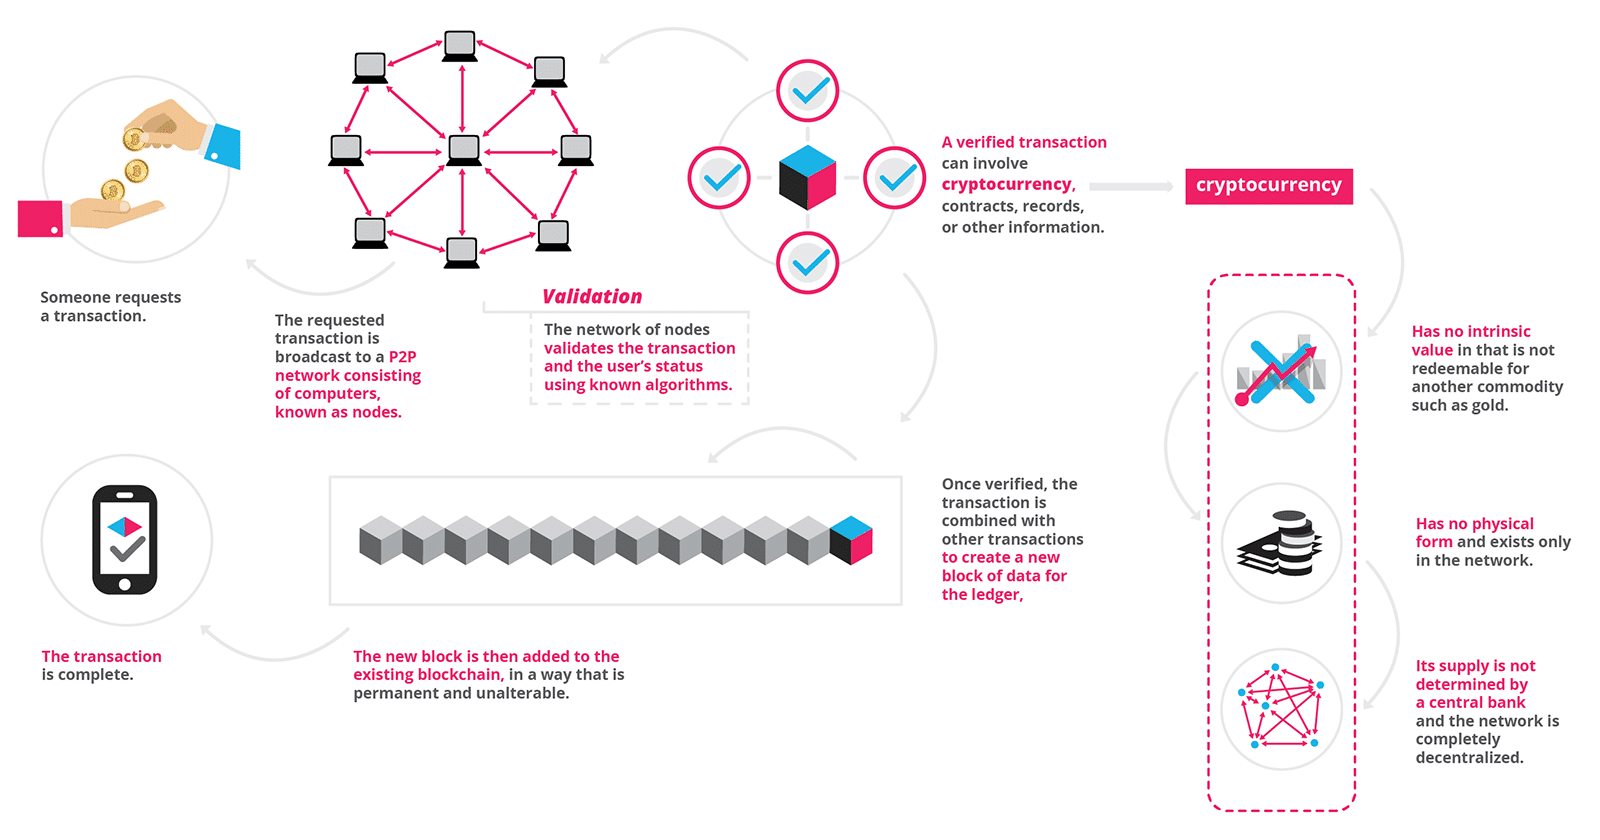
\includegraphics[width=16cm]{infographics0517-01-1.png}
  \caption{An abstract of a blockchain system \cite{whatIsBlockgeeks}}
  \label{blockchainAbstract}
\end{figure}

\subsection{Docker}
\label{docker}
Docker and Docker Composer are essential for the developing of this project. This technology is being used to run Hyperledger Fabric. Different parts, modules, of the system are mounted on Docker containers. All of those containers know about each other and intercommunicate. This system is also known as Fabric.

	Docker containers are similar to a virtual machines. Alike resource isolation and allocation benefits, however, containers are more portable and efficient since they virtualize the OS instead of hardware.\cite{dockerContainer} Figure \ref{dockerEnvironment} shows an abstraction of where Docker containers take place in the software architecture when running.

\begin{figure}[h]
\centering
  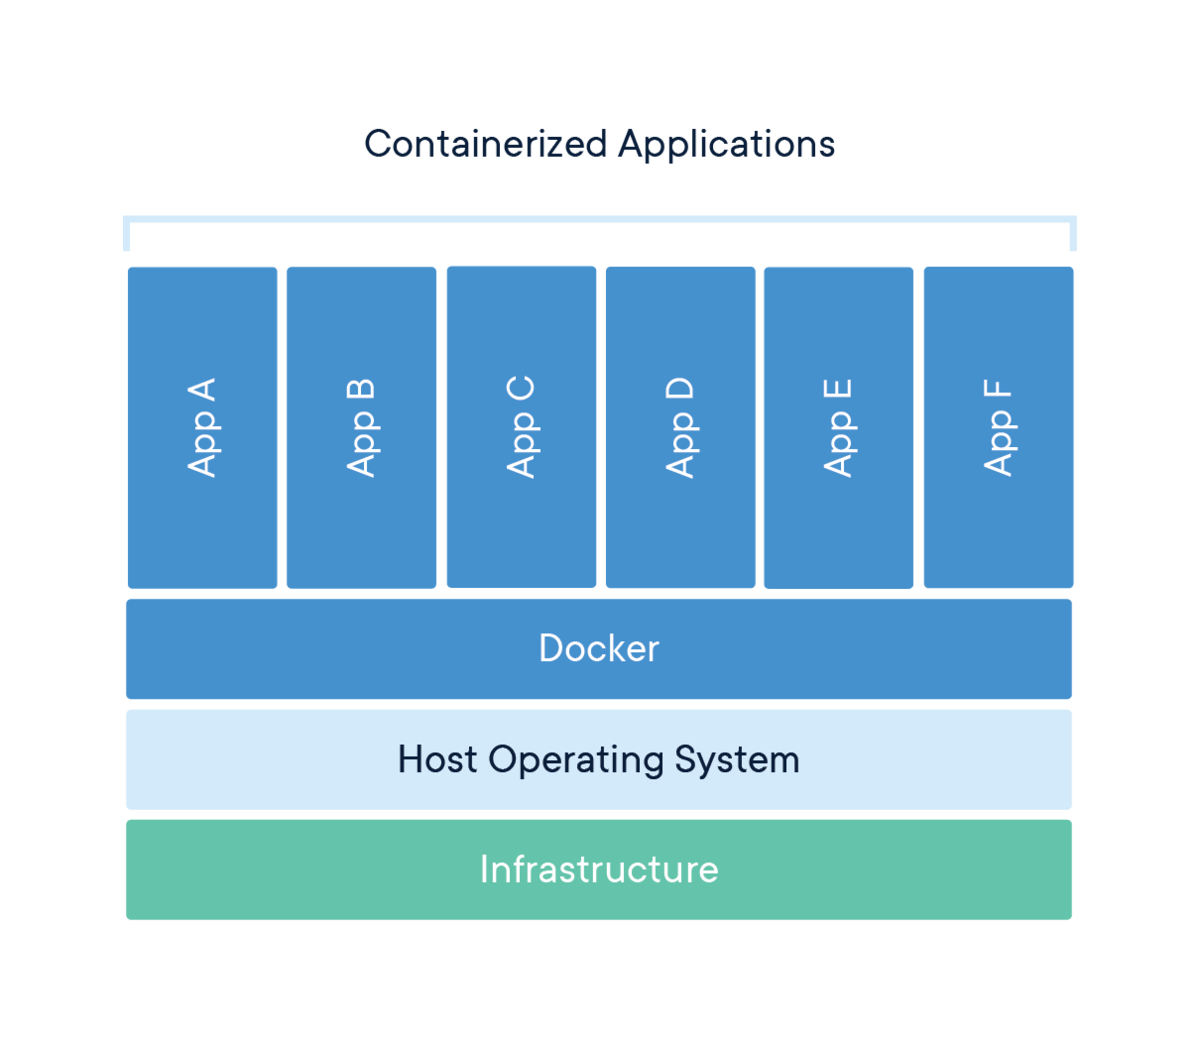
\includegraphics[width = 16cm]{container-what-is-container.png}
  \caption{ Containerized applications \cite{dockerContainer}}
  \label{dockerEnvironment}
\end{figure}

\section{Permissioned Blockchain}
\label{permissionedBlockchain}
A blockchain where the peers need to meet certain requirements to enter the network where they can perform certain actions is called permissioned. These systems are more attractive for the business and enterprise because they are faster and more cost-effective. Another feature that is appealing for those clients is the role system. That way actors, that all of the companies trust, can be the endorsers, the ones to validate the transactions. The feature could also be used to classify different players into respective roles. This can give a particular system a better clarification and simplicity around executing different tasks. 

	It is not as decentralized system as permissionless blockchain, however the tradeoff is acceptable enough for businesses to prefer it. The processes of “Anti-Money Laundering” and “Know Your Customer” require that service providers can confirm a peer’s legal identity and give clearance to make a transaction. The adoption of these processes in permissionless blockchain would be wrong, since they can illuminate who this peer is, thus breaking the promised anonymity. On another note, a permissioned blockchain can have larger volume of transactions compared to a public one. 
	
What’s more, many prefer permissioned blockchains for supply chain. Since only the peers inside the blockchain can see what is happening on the path of a material to its final destination. And the tracking data can travel much faster, due to the simplified verification and less peers. 


\subsection{Hyperledger Fabric}
\label{hyperledgerFabric} 
Hyperledger is a group of open source projects focused around cross-industry distributed ledger technologies. Hosted by The Linux Foundation, collaborators include industry leaders in technology, finance, banking, supply chain management, manufacturing, and IoT.

	Fabric is one of those open source projects. It is a modular distributed ledger, which makes it highly customizable and adaptable to a variety of ideas and restrictions. The main scope of this undergraduate project is to test how functional and useful Fabric can be in different business and science situations. Is it making some of the use cases in those fields cheaper and more secure?
	
The feature which makes Fabric the perfect choice is that it can create different communication channels between different peers. Some of those channels could be for contract making between a supplier and a buyer. If a supplier has a favourite customer, he or she may give an exclusive deal. However, if everyone see this exclusive deal, then the business of the supplier would break down. That’s why this exclusive deal could exist in a confidential channel, one that only the two of them can see. 

	This Hyperledger project is a preferred platform mainly because of its adaptability to different use cases. One interesting feature, and main reason for the self-sovereign use case, is that Fabric supports zero-knowledge proof (ZKP). What this means is that it allows a peer to assure itself in front of a verifier without having to show any private data. This gives authority to ZKP to offer anonymous authentication for clients in their transactions. \cite{li2018fppb}
	
	The act of communication between different peers from different organizations (or groups) is through channels. These channels can be public or confidential. The communication inside works based on the chaincode, the smart contract. All of the logistics and functionality of a new blockchain application is based on it’s smart contracts. That is why they are extremely important and main object of interest in this undergraduate project. 

\section{Successful projects made with Hyperledger Fabric}
\label{successfulFabric}

\subsection{Altoros}
\label{altoros}
Altoros is a software company that delivers different solutions. One of the problems their customers have is issuing bonds. The customer, Russia's National Settlement Depository (NSD), wanted a system that allows automate bond placement and accounting with blockchain, while minimizing risks of reconciliation and ensuring transparency. The reason they chose Fabric is for its support of confidential transactions and resilience in the production environment. \cite{altoros}

	What they did was to customize Fabric as needed for the different roles and actions. They set up four different channels so the communication,data transferring, between the peers and the NSD could be safe and secure. Every channel has its own chaincode ( smart contract) that is basically the logistics behind the given channel.
	
	One of the challenges they had was that the REST API was still in development. Fortunately, this is not the case anymore. Another challenge is that Fabric does not support cross-channel transactions. \cite{altorosDemo}
	
	The benefits of choosing Fabric are: 
	\begin{itemize}
	
\item Faster transactions compared to the traditional solution, where a lot of data exchanging has to be done through a middleman. Thus, not only making it faster but also cheaper. 
\item Minimizing fraud in a secure trusted network. The permissioned feature does not allow for anyone that does not meet the requirements to monitor what’s happening into the world ledger. What’s more because of the non cross-channel transactions, a peer could observe only the channels he is using. And even when he or she is inspecting another peer’s transaction, because of the encryption, he or she would not get any valuable information. 
\item Reduces expenses of the bond issuer by making the process faster and simplified
	\end{itemize}

\subsection{Verify.Me}
\label{verifyMe}
SecureKey is a company providing identity and authentication provider for simplified access to online services and applications. They are using trusted providers such as banks, telcos and governments to make their clients assert identity information and connect to critical online services with digital credentials.

After the government of Canada recognized their problem sending private data to a citizen, they asked for a solution. SecureKey responded to this call in collaboration with IBM with a blockchain based solution. It is a mobile app, that allows the user to connect different types of services providing only specific data. So what happens is the user connects to the blockchain through the phone. Then, it connects with the service actors. It is important to note that in the phone there are only pointers to the data and not the data itself. Whenever a person is sharing his or her identity with the new service he or she can see exactly what information is asked to be provided. \cite{verifyMe}

	The SIM card is used as an anchor of trust. Since the system is
private and permissioned blockchain, only trusted actors like banks and government can write on it. Upon losing or breaking the phone, the creators reassure that is easy to recover what’s lost. 
Again, here one of the main reasons to choose Fabric for the development of this service is mainly - the adaptability of the platform and the zero-knowledge proof supported concept. \cite{verifyMeDemo}

The benefits of using Fabric are : 
\begin{itemize}
\item Data integrity 
\item Security and resiliency
\item No central database or honeypots 
\item No central point of failure
\item Cannot track user across relying parties; privacy of the data
\item Cost efficient due to simplifying the process
\end{itemize}
Cons: 
\begin{itemize}
\item New - open standards needed 
\end{itemize}

\subsection{TradeLens}
\label{tradelens}

	TradeLens is a company founded by collaborative work of Maersk and IBM. Maersk is an integrated container logistics company working on improving the supply chain area. The idea is to make the shipping process cost-efficient, faster and in respect to accessing the needed documents - simpler.
	 
	For this task, the collaboration is combining their technical and specialized knowledge to build a system on top of Hyperledger Fabric. What they created is a network, that tracks the supply chain - the documents needed for starting a shipping process, the deal that is made, the location of the containers.
	 
	To participate, a user has to pay a price to enter the network. Still it is not confirmed what the requirements are. However, once a user decides to enter he will experience something way different from the usual way of things. Due to the blockchain technology, a user can check a block on the blockchain to track the location of the container or any other process involved. The usual way for this simple task would be to request this information from a middleman. TradeLens are saying they can reduce the paperwork and the need of a mediators, saving lots of time and money in the process. \cite{tradeLensFounders}
	
	It is important to be mentioned that TradeLens is not fighting the frauds. If a user input false data at start,that seems to be correct to the endorsement parties, the system won’t be able to catch it. So the network helps to have less fraud, but it is more of a side effect rather than main function.
	
	Another great use of this system is that, according to the World Trade Organization, simplifying the supply chain will not only reduce costs, but also help developing countries to increase their export by more than 30\% . [16]

%%%%%%%%%%%%%%%%%%%%%%%%%%%%%%%%%%%  Problem description and analysis 
 %%%%%%%%%%%%%%%%%%%%%%%%%%%%%%%%%%%

\chapter{Problem description and analysis}

\label{approach}
The problem that this project will address is about the structure of the Hyperledger Fabric blockchain platform. This new technology has the potential to save a lot of resources and ease the hardship of data management and accessibility.  

 	The second part of this project will try to cover the understanding of the digital identity and creating a prototype. 
\section{How Hyperledger Fabric works}
\label{fabricWorks}
Researching how the smart contracts on this platform work will give a representation of how the blockchain is being managed and controlled. Understanding the flow of work will show the opportunities that this technology gives and the restrictions that have to be taken into account upon developing a solution. The greatest opportunity lies in the decentralized nature of the technology and its integrity. The project has an aim to show why Hyperledger should be considered for future solutions, in various fields, and give a example.

As discussed in 2.2.1, Fabric is very adaptable and customizable. The approach that I will take is to follow the steps of the official tutorial. This will give me knowledge how fabric is mounted on Docker and how the system is run. From then on, I will be able to start customizing the network and change different modules. I shall see if the changes are giving the expected results, or maybe the system is behaving better or worse.
 
Next will be the additional parties. Is it harder, more resourceful, to have a new peer enter the system, rather than having all the parties starting at the beginning? How is the system reacting to the new peer, is every public channel giving him all of the information about the previous transactions, or is there a threshold somewhere? 

How powerful must be the hardware to support such a system? In permissionless blockchain, everybody can be supporting the system nodes, miners, or just to be peers. However, as I mentioned it already, this is not the case with the permissioned one. Should this become a real problem in the future, if the transactions and the data are exceeding the expectations and estimations of the developers? 


\section{Self-sovereign identity}
\label{selfIdentity}
To understand self-sovereign identity, a research of the identity itself is needed. Firstly, it is the philosophical aspect of the word. Secondly, it will be the idea of the digital meaning and how the two differ. 

I will seek for an answer if this new blockchain technology can shrink the difference between normal and cybernated identity and how. But more importantly, with this project I will answer if it is going to be cost-effective enough, so that the world could start considering the option of transitioning into this kind of a system

Lastly, I will consider the aspect of security of the identity. Is this system going to be secure enough to be used by real peers? Is it going to be able to withstand the traffic and data stored?


%%%%%%%%%%%%%%%%%%%%%%%%%%%%%%%%%%% Citations %%%%%%%%%%%%%%%%%%%%%%%%%%%%%%%%%%

\bibliographystyle{abbrv}

\bibliography{ref}

\end{document}
